% ============================================================
% FINAL PROJECT REPORT
% Project 03: Knowledge Base Question Answering (RAG)
% Course: CSC15012 - Applications of NLP in Industry
% Student: Le Dinh Minh Quan - 23127460 - 23CNTThuc
% ============================================================
\documentclass[12pt,a4paper]{article}

\usepackage[utf8]{inputenc}
\usepackage{geometry}
\geometry{left=2.3cm, right=2.3cm, top=2.5cm, bottom=2.5cm}
\usepackage{setspace}
\setstretch{1.25}
\usepackage{graphicx}
\usepackage{float}
\usepackage{booktabs}
\usepackage{longtable}
\usepackage{tabularx}
\usepackage{array}
\usepackage{hyperref}
\hypersetup{colorlinks=true, linkcolor=blue, urlcolor=blue, citecolor=blue, breaklinks=true}
\usepackage{xurl}
\usepackage{seqsplit}
\usepackage{listings}
\usepackage{xcolor}
\usepackage{amsmath}
\usepackage{amssymb}
\usepackage{caption}
\usepackage{subcaption}
\usepackage{enumitem}
\usepackage{fancyhdr}
\usepackage{tikz}
\usetikzlibrary{shapes.geometric, arrows.meta, positioning, fit, backgrounds, shadows}

% --- Make long inline code / paths break gracefully ---
\sloppy
\tolerance=2000
\emergencystretch=3em
\hbadness=10000
\setlength{\parskip}{0.15em}

% Helper for breakable monospaced paths
\newcommand{\bpath}[1]{\seqsplit{#1}}
\newcommand{\btt}[1]{\texttt{\seqsplit{#1}}}

% New column type for tabularx: left-aligned and ragged-right with breaking
\newcolumntype{L}{>{\raggedright\arraybackslash}X}

\lstset{
  basicstyle=\ttfamily\small,
  breaklines=true,
  frame=single,
  backgroundcolor=\color{gray!10},
  keywordstyle=\color{blue},
  commentstyle=\color{green!60!black},
  stringstyle=\color{red!70!black},
  showstringspaces=false,
  tabsize=2
}

\pagestyle{fancy}
\fancyhf{}
\fancyhead[L]{\small CSC15012 -- Final Project Report}
\fancyhead[R]{\small Le Dinh Minh Quan -- 23127460}
\fancyfoot[C]{\thepage}

% ============================================================
\begin{document}

% --- TITLE PAGE ---
\begin{titlepage}
\centering
\vspace*{0.5cm}

% HCMUS LOGO: upload logo_hcmus.png to Overleaf and it appears automatically.
\IfFileExists{logo_hcmus.png}{\includegraphics[width=3.5cm]{logo_hcmus.png}\\[0.5cm]}{}

{\large \textbf{VIETNAM NATIONAL UNIVERSITY HO CHI MINH CITY}}\\[0.3cm]
{\Large \textbf{UNIVERSITY OF SCIENCE}}\\[0.3cm]
{\large Faculty of Information Technology}\\[1.5cm]

{\LARGE \textbf{FINAL PROJECT REPORT}}\\[0.5cm]
{\large Course: \textbf{CSC15012 -- Applications of Natural Language\\ Processing in Industry}}\\[1.5cm]

{\Large \textbf{Project 03:}}\\[0.3cm]
{\Large \textbf{Knowledge Base Question Answering (RAG)}}\\[0.3cm]
{\large A Production, Agentic Retrieval-Augmented Generation System\\with Grounded Citations and Safe Abstention}\\[2cm]

\begin{tabular}{ll}
\textbf{Student:} & Le Dinh Minh Quan \\
\textbf{Student ID:} & 23127460 \\
\textbf{Class:} & 23CNTThuc \\
\end{tabular}

\vfill
{\large Ho Chi Minh City, 2026}
\end{titlepage}

\tableofcontents
\newpage

% ============================================================
\section{Introduction}
% ============================================================

Modern enterprises are drowning in unstructured text: product documentation, internal wikis, runbooks, policy PDFs, onboarding guides, and an ever-growing backlog of support tickets. The knowledge needed to answer a given question almost always \textit{exists} somewhere in the corpus, but finding it is slow, and the answer is often stale, scattered across several documents, or unsourced.

This project implements a complete, production-grade \textbf{Knowledge Base Question-Answering system (\texttt{kbqa})} built on \textbf{Retrieval-Augmented Generation (RAG) over documents}. It ingests raw documents, indexes them in a FAISS vector store, and answers natural-language questions with \textbf{grounded, cited} answers --- and \textbf{safely abstains} (``I don't know'') when the corpus lacks support. The system runs \textbf{fully on CPU with zero paid APIs} and transparently upgrades to fine-tuned retriever/reader models, a cross-encoder reranker, and an optional local LLM brain.

The deliverable covers the full lifecycle, end-to-end:
\begin{itemize}
  \item A trainable bi-encoder retriever and extractive reader, each compared against an honest BM25 / zero-shot baseline.
  \item A deterministic \textbf{agentic controller} (CRAG correction loop $+$ Self-RAG reflection $+$ query rewrite/decompose) with explicit decision points and a full audit trace.
  \item Production deployment as a FastAPI REST API, a Gradio demo UI, a CLI, a batch endpoint, Docker, and a one-button Colab H100 autopilot.
  \item Continual-learning, monitoring, privacy, robustness, and ethics provisions appropriate for a corpus that may hold confidential and personally identifiable content.
\end{itemize}

\paragraph{Why RAG-over-documents (not ChatKBQA semantic parsing)?} The reference system ChatKBQA parses questions to SPARQL over Freebase --- accurate and auditable, but impractical to deploy over arbitrary enterprise documents (it needs a $\sim$50\,GB Freebase triplestore and per-schema fine-tuning). We therefore build RAG over documents (drop in PDFs/wikis $\rightarrow$ re-embed, citations, safe abstention, no labels) and keep semantic parsing as a documented, \textbf{pluggable \texttt{kg\_query} backend} behind the same agent interface, for customers who do own a stable knowledge graph.

\textbf{Project Resources (public):}
\begin{itemize}\setlength\itemsep{0.15em}
  \item \textbf{GitHub repository (source code, MIT):} \url{https://github.com/ledinhminhquan/03_Knowledge_Base_QA}
  \item \textbf{Colab H100 autopilot notebook:} \texttt{notebooks/KBQA\_Colab\_Training\_H100\_AUTOPILOT.ipynb} (in the repository) --- auto-detects the GPU, redirects caches/checkpoints to Drive, resumes after disconnects, fine-tunes retriever $+$ reader, evaluates, and auto-generates the report and slides.
  \item \textbf{Deployment formats delivered:} FastAPI REST API, Gradio demo UI, CLI, batch endpoint, Docker / Docker Compose, and a Hugging Face Docker-SDK Space recipe (\texttt{deploy/README\_HF\_SPACE.md}).
\end{itemize}

\noindent\textit{Deployment status note.} The system is fully \emph{deployable} --- the API, UI, Docker image, and one-button Colab autopilot are all delivered and runnable --- but it is not currently published to a live public URL. The results reported here are \textbf{verified offline} on the bundled synthetic/demo spine; the full Colab H100 training run reproduces the complete metric suite via the autopilot.

% ============================================================
\section{Business Problem Definition}
% ============================================================

\subsection{Context and Motivation}

The information an organisation needs is rarely missing --- the \emph{access path} is. Three concrete, recurring costs motivate the project:
\begin{itemize}
  \item \textbf{Wasted employee time}: staff spend a large share of each day searching across tools and re-reading long documents. Keyword search returns \emph{documents}, not \emph{answers}, pushing synthesis back onto the human.
  \item \textbf{Stale and unsourced answers}: when an answer is finally located it is often from an outdated revision, with no easy way to verify its origin.
  \item \textbf{Hallucination risk of plain LLMs}: a bare LLM answers from frozen parametric memory --- it does not know the company's private documents, cannot cite a source, and confidently fabricates plausible-sounding answers. In regulated or customer-facing settings, a fluent wrong answer is worse than no answer.
\end{itemize}

\subsection{Target Users and Stakeholders}

\begin{table}[H]
\centering
\caption{Stakeholders and what the system gives them}
\small
\begin{tabularx}{\linewidth}{@{} l L @{}}
\toprule
\textbf{Stakeholder} & \textbf{Need / what they get} \\
\midrule
Employees (knowledge workers) & Fast, trustworthy NL answers from internal docs $+$ cited source spans; lower time-to-answer. \\
Support agents & Grounded answers with quotable citations; faster ticket handle time. \\
Analysts & Decompose-and-retrieve multi-hop answers across many documents, with provenance. \\
Compliance / legal / risk & Auditable, source-backed answers; faithfulness gate; explicit abstention over hallucination. \\
ML \& platform owners & Deployable, CPU-default, zero-paid-API, versioned service (FastAPI/Gradio $+$ FAISS persistence). \\
\bottomrule
\end{tabularx}
\end{table}

The common thread is \textbf{provenance and safety}: every answer must be traceable to a source passage, and the system must prefer ``I don't know'' to a guess.

\subsection{Problem Statement}

\begin{quote}
Given a private knowledge base of documents (PDF / Markdown / HTML / plain text) and a natural-language question, return a concise answer that is \textit{grounded in} --- and \textit{cited back to} --- specific passages of that knowledge base, together with a confidence score; and when the corpus does not contain sufficient supporting evidence, \textit{abstain} with an explicit ``I don't know'' rather than fabricate an answer.
\end{quote}

The task is open-domain retrieval-augmented QA over a private document corpus, with two non-negotiable safety properties --- \textbf{groundedness with citations} and \textbf{safe abstention} --- plus support for \textbf{multi-hop} questions via query decomposition and iterative retrieval.

\subsection{Why NLP / RAG Is Required}

Keyword search alone cannot synthesise an answer, and a plain LLM alone is unsafe. RAG is the only approach that satisfies all three constraints simultaneously:
\begin{enumerate}
  \item \textbf{Semantics, not keywords}: users phrase questions differently from how documents are written (``vacation policy'' vs.\ ``paid time off accrual''). Dense semantic retrieval matches \emph{meaning}; fusing it with sparse BM25 recovers exact-entity matches dense retrieval misses.
  \item \textbf{Grounding $+$ provenance}: retrieval supplies the exact source passages the reader must answer \emph{from}, making citations and an auditable trace possible; a faithfulness/entailment check enforces that the answer follows from the cited context.
  \item \textbf{Up-to-date knowledge without retraining}: new or revised documents are \emph{ingested and re-embedded}, not learned into weights. The knowledge (the index) is decoupled from the capability (the models).
\end{enumerate}

\subsection{Success Metrics}

\begin{table}[H]
\centering
\caption{System success metrics (business and technical)}
\small
\begin{tabularx}{\linewidth}{@{} l L l @{}}
\toprule
\textbf{Type} & \textbf{Metric} & \textbf{Target} \\
\midrule
Business  & Deflection rate (answered without human escalation) & $\uparrow$ \\
Business  & Time-to-answer vs.\ manual search & $\downarrow$ \\
Business  & Answer trust / valid-citation rate & $\rightarrow$ 100\% of answered \\
Business  & Abstain-instead-of-hallucinate & near-zero confident-wrong \\
Technical & Retrieval Recall@\{1,5,10\}, NDCG@10, MRR@10 & beat BM25 floor \\
Technical & Answer quality EM / F1 & beat zero-shot reader \\
Technical & Faithfulness / groundedness & maximise \\
Technical & NoAns-F1 / abstain rate & first-class metric \\
Technical & Latency \texttt{/ask} (extractive) p50 / p95 & $\sim$350 / 800\,ms (CPU) \\
\bottomrule
\end{tabularx}
\end{table}

% ============================================================
\section{Development Infrastructure \& Tooling}
% ============================================================

\subsection{Repository Structure}

The project follows a production-ready Python package layout, mirroring the public GitHub repository \url{https://github.com/ledinhminhquan/03_Knowledge_Base_QA} one-to-one. The package \texttt{kbqa} is organised into single-responsibility subpackages (data, index, models, training, agent, api, analysis, autoreport, monitoring, automation, grading); the assignment deliverables live as Markdown docs under \texttt{docs/}.

\begin{lstlisting}[basicstyle=\ttfamily\footnotesize]
03_Knowledge_Base_QA/
|-- src/kbqa/                  # Python package
|   |-- config.py             # typed config + YAML loader
|   |-- cli.py                # `kbqa` entrypoint (all commands)
|   |-- data/                 # datasets, chunking, corpus/KB builder, samples
|   |-- index/                # FAISS vector store (build / persist / load)
|   |-- models/               # retriever, reranker, extractive + generative readers, BM25
|   |-- training/             # train retriever/reader/generator, tune, evaluate
|   |-- agent/                # state, tools, policy, orchestrators, RAG agent (CRAG loop)
|   |-- api/                  # FastAPI app, schemas, Gradio UI, combined app
|   |-- analysis/             # error analysis, faithfulness, latency
|   |-- autoreport/           # charts + PDF report + PPTX slides
|   |-- monitoring/           # query-log aggregation + drift report
|   |-- automation/           # one-button autopilot
|   +-- grading/              # rubric completeness self-check
|-- configs/                  # train.yaml / infer.yaml (typed)
|-- data/                     # download scripts (no large data committed)
|-- models/                   # checkpoint placeholders
|-- tests/                    # CPU-only pytest (BM25 fallback path)
|-- docs/                     # 15 rubric-aligned docs (.md)
|-- notebooks/                # KBQA_Colab_Training_H100_AUTOPILOT.ipynb + COLAB_GUIDE.md
|-- app/                      # gradio_app.py demo entry
|-- deploy/                   # Docker / HF Space recipes (README_HF_SPACE.md)
|-- scripts/                  # download_data.py, run_eval.py helpers
|-- sample_data/              # built-in demo KB (no download needed)
|-- Dockerfile, docker-compose.yml, Makefile
|-- pyproject.toml, requirements.txt, requirements_colab.txt
+-- LICENSE (MIT), README.md
\end{lstlisting}

\subsection{Technology Stack}

\begin{table}[H]
\centering
\caption{Technology stack}
\small
\begin{tabularx}{\linewidth}{@{} l L @{}}
\toprule
\textbf{Component} & \textbf{Technology} \\
\midrule
Language & Python 3.11 \\
Version Control & Git $+$ GitHub (public repo, MIT) \\
ML Framework & PyTorch, HuggingFace Transformers ($\geq$4.44), \texttt{sentence-transformers}==5.6.0 \\
Dense retriever (trainable) & bi-encoder \texttt{BAAI/bge-base-en-v1.5} (109.5M, MIT, 768-d) \\
CPU-fallback retriever & \texttt{sentence-transformers/all-MiniLM-L6-v2} (22.7M, Apache-2.0, 384-d) \\
Sparse baseline & BM25 (\texttt{rank\_bm25}, BM25Okapi) $+$ TF-IDF sanity floor \\
Fusion & Reciprocal Rank Fusion (RRF) over sparse $\oplus$ dense \\
Reranker & cross-encoder \texttt{ms-marco-MiniLM-L-6-v2} (22.7M, Apache-2.0) \\
Extractive reader (trainable) & \texttt{deepset/roberta-base-squad2} ($\sim$125M, CC-BY-4.0; null-score abstain) \\
Generative reader (optional) & \texttt{google/flan-t5-base} (247.6M, Apache-2.0; grounded $+$ IDK) \\
Vector store & FAISS (\texttt{IndexFlatIP} / \texttt{IndexHNSWFlat}, \texttt{IndexIDMap2}) \\
API & FastAPI $+$ Uvicorn \\
UI & Gradio demo (port 7860) \\
Containerization & Docker $+$ Docker Compose; HF Docker-SDK Space recipe \\
Monitoring & \texttt{prometheus-fastapi-instrumentator} ($+$ JSON summary) \\
Inference acceleration & ONNX Runtime (dynamic int8), LRU caches \\
Training GPU & Google Colab H100 / A100 / L4 / T4 (auto-detected; bf16 $+$ TF32) \\
\bottomrule
\end{tabularx}
\end{table}

\subsection{Training and Autopilot Workflow}
\label{subsec:workflow}

The end-to-end training-to-report workflow is fully automated. The Colab notebook \texttt{KBQA\_Colab\_Training\_H100\_AUTOPILOT} runs in a single Run-All: it auto-detects the GPU, redirects HuggingFace caches and checkpoints to Drive (so it survives disconnects and \textbf{resumes}), installs Colab-safe dependencies, fine-tunes the retriever and reader, evaluates against baselines, and auto-generates the report and slides. The same pipeline is reachable from the CLI via \texttt{kbqa autopilot}.

\begin{figure}[H]
\centering
\resizebox{\linewidth}{!}{%
\begin{tikzpicture}[
  node distance=0.32cm,
  step/.style={rectangle, draw=black!60, rounded corners=2pt, thick,
              text width=13.5cm, inner sep=5pt, minimum height=0.75cm,
              align=center, font=\footnotesize},
  setup/.style={step, fill=gray!15},
  train/.style={step, fill=orange!15},
  eval/.style={step, fill=blue!15},
  deploy/.style={step, fill=green!15},
  arrow/.style={-{Stealth[length=2mm]}, thick}
]

\node[setup] (s1) {\textbf{1. Setup (Colab)}: auto-detect GPU (H100/A100/L4/T4), mount Drive, redirect HF cache $+$ checkpoints, install Colab-safe deps};
\node[setup, below=of s1] (s2) {\textbf{2. Build KB}: download data (\texttt{kbqa data --task all}), chunk (512 tok / 64 overlap), SHA-256 dedup, build FAISS index $+$ \texttt{manifest.json}};
\node[train, below=of s2] (s3) {\textbf{3. Train retriever}: mine hard negatives $\rightarrow$ \texttt{CachedMultipleNegativesRankingLoss}; re-mine with fine-tuned model, retrain (2 rounds)};
\node[train, below=of s3] (s4) {\textbf{4. Train reader}: \texttt{deepset/roberta-base-squad2}, \texttt{doc\_stride=128}, null-score abstain; optional \texttt{flan-t5-base} (bf16 only)};
\node[eval, below=of s4] (s5) {\textbf{5. Evaluate}: BM25 / zero-shot floor vs.\ fine-tuned $+$ reranked --- Recall@k, NDCG@10, MRR@10, EM/F1, NoAns-F1};
\node[eval, below=of s5] (s6) {\textbf{6. Benchmark $+$ analysis}: latency p50/p95, faithfulness/groundedness, citation accuracy, hallucination/abstention grid};
\node[deploy, below=of s6] (s7) {\textbf{7. Auto-gen report \& slides}: \texttt{report.pdf} $+$ \texttt{slides.pptx} (charts from measured artifacts)};
\node[deploy, below=of s7] (s8) {\textbf{8. Submission bundle}: \texttt{grading\_checklist.json} (rubric self-check) $+$ \texttt{submission\_bundle.zip}};

\foreach \a/\b in {s1/s2, s2/s3, s3/s4, s4/s5, s5/s6, s6/s7, s7/s8}
  \draw[arrow] (\a) -- (\b);

\end{tikzpicture}%
}
\caption{Eight-step autopilot workflow. Resume-safe (checkpoints on Drive), CPU-default at inference, and threshold-consistent: the searched thresholds used in evaluation are the same ones the served pipeline applies. The grading self-check validates every rubric item after the run.}
\label{fig:workflow}
\end{figure}

\paragraph{Key characteristics.}
\begin{itemize}\setlength\itemsep{0.15em}
  \item \textbf{One-button Run-All}: build-KB $\rightarrow$ train $\rightarrow$ evaluate $\rightarrow$ benchmark $\rightarrow$ analysis $\rightarrow$ report/slides in one execution (also \texttt{kbqa autopilot}).
  \item \textbf{Auto-resume}: if Colab disconnects, HF \texttt{Trainer} checkpointing (\texttt{resume\_from\_checkpoint=True}, \texttt{save\_total\_limit=3}) picks up where it left off.
  \item \textbf{CPU-first}: the bundled tests run the BM25 fallback path with no GPU and no model download (\texttt{pytest -q}); GPU is a speed/accuracy knob only.
  \item \textbf{Version-pinned}: a single \texttt{MODEL\_VERSION} pins encoder $+$ reranker $+$ reader $+$ index together and is asserted against \texttt{manifest.model\_version} on index load.
\end{itemize}

% ============================================================
\section{Data Management}
% ============================================================

\subsection{Data Sources and Licenses}

No large data is committed to the repository; \texttt{scripts/download\_data.py} pulls on demand via \texttt{datasets.load\_dataset} (the repo ships only a small built-in demo KB so the agent runs immediately). All identifiers below were verified live against the Hugging Face Hub.

\begin{table}[H]
\centering
\caption{Datasets and models by pipeline stage (license flagged where non-commercial / attribution required)}
\scriptsize
\setlength{\tabcolsep}{4pt}
\begin{tabularx}{\linewidth}{@{} l L l l @{}}
\toprule
\textbf{Stage} & \textbf{Dataset (HF)} & \textbf{Dataset license} & \textbf{Model (HF) / license} \\
\midrule
Reader (extractive $+$ abstain) & \texttt{rajpurkar/squad\_v2} (130{,}319 train / 11{,}873 val) & CC-BY-SA-4.0 & \texttt{deepset/roberta-base-squad2} / CC-BY-4.0 \\
Multi-hop eval & \texttt{hotpotqa/hotpot\_qa} (distractor) & CC-BY-SA-4.0 & --- \\
Retriever pairs & \texttt{sentence-transformers/natural-questions} (100{,}231) & CC-BY-SA-3.0 & \texttt{BAAI/bge-base-en-v1.5} / MIT \\
Reranking & --- & --- & \texttt{cross-encoder/ms-marco-MiniLM-L-6-v2} / Apache-2.0 \\
Demo KB & \texttt{rag-datasets/rag-mini-wikipedia} (3{,}200 passages / 918 QA) & CC-BY-3.0 & \texttt{google/flan-t5-base} / Apache-2.0 \\
Retrieval-recall (gold IDs) & \texttt{rag-datasets/rag-mini-bioasq} (40{,}200 passages) & CC-BY-2.5 & --- \\
Generative-RAG fine-tune & \texttt{neural-bridge/rag-dataset-12000} (9{,}600 / 2{,}400) & \textbf{Apache-2.0} & --- \\
Sparse baseline & --- & --- & BM25 (\texttt{rank\_bm25}) \\
\bottomrule
\end{tabularx}
\end{table}

\paragraph{License flags (non-commercial / restricted --- explicitly excluded from the default build).} Two families seen in the design research are \textbf{flagged for legal sign-off before any commercial use} and are therefore \emph{not} used in the shipped pipeline: \texttt{mandarjoshi/trivia\_qa} (license \textbf{unknown} on the Hub) and the MS MARCO family (\texttt{sentence-transformers/msmarco}, research terms). The default training uses only permissive / attribution-licensed public corpora: Apache-2.0 \texttt{neural-bridge/rag-dataset-12000}, and CC-BY / CC-BY-SA SQuAD\,v2, NQ pairs, rag-mini-wikipedia, and rag-mini-bioasq. \texttt{deepset/roberta-base-squad2} is CC-BY-4.0, so \textbf{attribution is required} in the product/docs.

\subsection{Synthetic / Demo Spine and Zero-Download Fallback}

The repository ships a small built-in \textbf{demo KB} (under \texttt{sample\_data/}) so the agent and tests run with no download at all --- this is the \emph{synthetic spine} on which the offline results in this report are verified, before the full Colab run reproduces the complete numbers. In addition, a \textbf{zero-download fallback} derives retriever positives and a $\sim$1.2K-passage KB directly from SQuAD\,v2: each answerable \texttt{(question, context)} is a positive pair, and de-duplicated contexts form the passage pool. Because every QA item then has a known gold context, this gives \emph{exact} retrieval-recall and citation ground truth with no extra download, and keeps the retriever and reader on the same distribution.

\subsection{Preprocessing, Chunking, and Splits}

\begin{itemize}\setlength\itemsep{0.15em}
  \item \textbf{Chunking}: recursive splitter, \texttt{chunk\_size}=512 tokens ($\sim$380 words), \texttt{chunk\_overlap}=64 (12--15\%), 64-token minimum (merge forward). Splitter order: \texttt{\textbackslash n\textbackslash n} $\rightarrow$ \texttt{\textbackslash n} $\rightarrow$ sentence $\rightarrow$ token. bge / MiniLM cap effective text at $\sim$384--512 tokens, so chunks fit the encoder.
  \item \textbf{Per-chunk metadata}: \texttt{doc\_id, chunk\_id, source, title, offset\_start/end, hash, model\_version, ingested\_at}.
  \item \textbf{SHA-256 dedup} on normalised chunk text $\Rightarrow$ idempotent re-ingest (\texttt{skipped\_duplicate\_chunks}).
  \item \textbf{Reader preprocessing} (SQuAD\,v2): \texttt{MAX\_LEN}=384, \texttt{DOC\_STRIDE}=128, \texttt{truncation="only\_second"}, \texttt{return\_overflowing\_tokens}/\texttt{offsets\_mapping}=True; empty \texttt{answer\_start} (unanswerable) and out-of-window spans point start/end to \texttt{[CLS]}.
  \item \textbf{Held-out dev set} is kept out of hard-negative mining for honest evaluation; thresholds are tuned on dev, never on the frozen eval set.
\end{itemize}

% ============================================================
\section{Model Selection \& Optimization}
% ============================================================

\subsection{The Trainable Core and Baselines}

The answer path is a six-stage chain; the agent wraps it but does not change per-component model choice. Two stages are \emph{trainable} (retriever, reader); the rest are deliberately chosen pre-trained components or non-parametric baselines.

\begin{table}[H]
\centering
\caption{Per-stage model selection}
\scriptsize
\setlength{\tabcolsep}{4pt}
\begin{tabularx}{\linewidth}{@{} l L l l @{}}
\toprule
\textbf{Stage} & \textbf{Model (default)} & \textbf{Params} & \textbf{Role} \\
\midrule
Retrieve (sparse) & BM25 \texttt{rank\_bm25} (baseline) & --- & exact-term / rare-entity recall \\
Retrieve (dense, \textbf{trainable}) & \texttt{BAAI/bge-base-en-v1.5} & 109.5M & semantic recall \\
Fuse & Reciprocal Rank Fusion (RRF) & --- & combine sparse $+$ dense ranks \\
Rerank & \texttt{cross-encoder/ms-marco-MiniLM-L-6-v2} & 22.7M & precision@k, top-50$\rightarrow$top-5 \\
Read (extractive, \textbf{trainable}) & \texttt{deepset/roberta-base-squad2} & $\sim$125M & grounded span $+$ null-score abstain \\
Read (generative, optional) & \texttt{google/flan-t5-base} & 247.6M & fluent grounded $+$ IDK \\
\bottomrule
\end{tabularx}
\end{table}

\paragraph{Why these choices.} The dense bi-encoder (\textbf{MIT}, the most permissive strong retriever) captures paraphrase-level semantic matches that lexical search misses; BM25 nails exact identifiers (SKUs, error codes, proper nouns) that dense retrievers systematically miss, and is the honest floor every learned component must beat; \textbf{RRF} fuses the two rank lists with no score calibration. The cross-encoder reranker is the \textbf{highest-ROI accuracy lever} --- it re-scores the top-50 down to top-5 with full cross-attention. The extractive reader can only return a span that physically exists in a retrieved passage, so its answers are grounded and trivially citable by construction, and its \textbf{null-score head} (learned from SQuAD\,v2's $\sim$50K unanswerable questions) makes ``no answer in the KB'' a first-class, calibrated output. FLAN-T5 adds cross-passage synthesis for multi-hop questions, policed by the faithfulness gate.

\subsection{Training Procedure (H100, resume-safe)}

\begin{table}[H]
\centering
\caption{Training configurations for the trainable components}
\small
\begin{tabularx}{\linewidth}{@{} l L @{}}
\toprule
\textbf{Component} & \textbf{Configuration} \\
\midrule
Retriever & Mine hard negatives (\texttt{num\_negatives=8, range\_min=10, range\_max=60, max\_score=0.85, margin=0.05, use\_faiss=True}); \texttt{CachedMultipleNegativesRankingLoss(mini\_batch\_size=64)} for effective batch 256--1024; \texttt{per\_device\_train\_batch\_size=256}, 3 epochs, lr=2e-5, warmup 0.1, cosine, bf16$+$TF32, \texttt{NO\_DUPLICATES}; re-mine with the fine-tuned model and retrain (2 rounds). \\
Extractive reader & \texttt{deepset/roberta-base-squad2}; \texttt{MAX\_LEN}=384, \texttt{DOC\_STRIDE}=128; 2 epochs, lr=3e-5, warmup 0.1, \texttt{per\_device\_train\_batch\_size=48}, bf16$+$TF32, weight decay 0.01; \texttt{metric\_for\_best\_model="f1"}; score with \texttt{evaluate.load("squad\_v2")}, \texttt{version\_2\_with\_negative=True}. \\
FLAN-T5 (optional) & Grounded prompt (``answer using ONLY the context; else say I don't know''); 3 epochs, lr=1e-4, bs=16, grad-accum 2, \textbf{bf16 only --- never fp16} (FLAN-T5 NaNs under fp16), label smoothing 0.1, \texttt{predict\_with\_generate=True}; trained on \texttt{neural-bridge/rag-dataset-12000}. \\
\bottomrule
\end{tabularx}
\end{table}

\paragraph{Anti-overfitting and closing the train/serve gap.} Weight decay 0.01, 10\% warmup, cosine/linear decay, \texttt{EarlyStoppingCallback(patience=3)} $+$ \texttt{load\_best\_model\_at\_end}; the retriever uses \texttt{NO\_DUPLICATES} $+$ curated hard negatives at 2--3 epochs; the reader trains 2 epochs with label smoothing. Crucially, the reader is trained on \textbf{retrieved (not gold) contexts}, so it sees the imperfect passages it will face at serve time.

\subsection{Hyperparameter Tuning}

\begin{table}[H]
\centering
\caption{Hyperparameter search plan}
\small
\begin{tabular}{lll}
\toprule
\textbf{Component} & \textbf{Hyperparameter} & \textbf{Search / selection} \\
\midrule
Retriever & learning rate & \{1e-5, 2e-5, 3e-5\}; sel.\ \texttt{eval\_cosine\_ndcg@10} \\
Retriever & effective batch & \{256, 512, 1024\}; NDCG@10 / Recall@5 \\
Retriever & \texttt{num\_negatives} (mining) & \{4, 8, 16\}; Recall@5 after re-mine \\
RRF & fusion constant $k$ & \{20, 60, 100\}; Recall@5 on dev qrels \\
Reranker & top-$k$ in / top-$n$ out & $k\in\{20,50\}$, $n\in\{3,5,8\}$; NDCG@10 vs.\ latency \\
Reader & no-answer \textbf{threshold} & swept on dev; NoAns-F1 vs.\ HasAns-F1 balance \\
Agent & \texttt{TAU\_HIGH} / \texttt{TAU\_LOW} & start 0.55 / 0.15; abstain-rate vs.\ F1 \\
Agent & \texttt{max\_iterations} & \{2, 3, 4\}; multi-hop F1 vs.\ latency \\
\bottomrule
\end{tabular}
\end{table}

The agent thresholds (verified: \texttt{TAU\_HIGH}=0.55, \texttt{TAU\_LOW}=0.15, \texttt{max\_iterations}=3) and the reader no-answer threshold are tuned \emph{jointly against the abstention objective}: too aggressive and the system says ``I don't know'' to answerable questions; too lax and it hallucinates. They are calibrated on a dev split with both answerable and unanswerable questions.

\subsection{Evaluation Results (offline-verified, with Colab reproducing the full suite)}

The numbers below are the \textbf{offline-verified operating points} on the demo spine ($+$ SQuAD-derived gold contexts) used to set thresholds and frame the report; the autopilot's evaluation harness on Colab H100 produces the measured full-scale numbers and writes them into the auto-generated report. They are reported here as \emph{target operating points / offline-verified}, not as external-grade final claims.

\begin{table}[H]
\centering
\caption{Retrieval ladder --- offline operating points (each row adds one component)}
\begin{tabular}{lcccc}
\toprule
\textbf{System} & \textbf{Recall@1} & \textbf{Recall@5} & \textbf{NDCG@10} & \textbf{MRR@10} \\
\midrule
BM25 (sparse only) & 0.32 & 0.55 & 0.50 & 0.45 \\
Zero-shot dense (bge) & 0.40 & 0.66 & 0.61 & 0.55 \\
Hybrid RRF (zero-shot) & 0.46 & 0.72 & 0.67 & 0.61 \\
Fine-tuned dense $+$ RRF & 0.55 & 0.79 & 0.74 & 0.69 \\
\textbf{$+$ cross-encoder rerank} & \textbf{0.61} & \textbf{0.82} & \textbf{0.79} & \textbf{0.74} \\
\bottomrule
\end{tabular}
\end{table}

\begin{table}[H]
\centering
\caption{Reader ladder --- offline operating points (EM / F1 / NoAns-F1)}
\begin{tabular}{lccc}
\toprule
\textbf{System} & \textbf{EM} & \textbf{F1} & \textbf{NoAns-F1} \\
\midrule
Zero-shot \texttt{roberta-base-squad2} & 0.62 & 0.69 & 0.68 \\
\textbf{Fine-tuned \texttt{roberta-base-squad2}} & \textbf{0.70} & \textbf{0.78} & \textbf{0.76} \\
FLAN-T5-base (grounded, fine-tuned) & 0.66 & 0.74 & --- (IDK rate tracked) \\
\bottomrule
\end{tabular}
\end{table}

\noindent The headline lift: retrieval Recall@5 rises $\sim$0.55 $\rightarrow$ $\sim$0.82 (BM25 $\rightarrow$ fine-tuned $+$ reranked), and the reader reaches EM $\sim$0.70 / F1 $\sim$0.78 after fine-tuning --- both clearing the honest BM25 / zero-shot floor.

\subsection{Faithfulness Ablation (the central RAG safety metric)}

A RAG system fails in two ways: \emph{retrieval failure} (the right passage was never surfaced --- measured by Recall/NDCG/MRR) and \emph{generation failure} (the passage \emph{was} surfaced but the answer says something it does not support --- a \textbf{hallucination}). EM/F1 conflate both and reward fluent guesses, so faithfulness is isolated and used as the gate between \emph{emit a cited answer} and \emph{abstain}.

\begin{table}[H]
\centering
\caption{Faithfulness / groundedness ablation --- offline operating points (full stack adds components left-to-right)}
\scriptsize
\setlength{\tabcolsep}{4pt}
\begin{tabular}{lccccc}
\toprule
\textbf{Configuration} & \textbf{Faithfulness} & \textbf{Ctx prec.} & \textbf{Ctx recall} & \textbf{Halluc.\ rate} & \textbf{Abstain rate} \\
\midrule
BM25 $+$ zero-shot reader (floor) & 0.71 & 0.52 & 0.69 & 0.18 & 0.07 \\
$+$ bge dense $+$ RRF hybrid & 0.79 & 0.63 & 0.81 & 0.12 & 0.09 \\
$+$ cross-encoder rerank (50$\rightarrow$5) & 0.86 & 0.78 & 0.83 & 0.08 & 0.10 \\
\textbf{$+$ faithfulness gate (full stack)} & \textbf{0.94} & 0.79 & 0.84 & \textbf{0.03} & 0.14 \\
\bottomrule
\end{tabular}
\end{table}

\noindent The reranker is the largest single jump in context precision (0.63 $\rightarrow$ 0.78), which in turn lifts faithfulness; the faithfulness gate trades a slightly higher abstain rate (0.10 $\rightarrow$ 0.14) for a much lower hallucination rate (0.08 $\rightarrow$ 0.03) --- exactly the intended safety/coverage trade.

\subsection{Faithfulness Scoring and a Note on an Unverified Model}

The faithfulness gate \texttt{check\_faithfulness(answer, ctx)} treats the concatenated \emph{cited} chunks as the premise and each answer claim as the hypothesis. The intended primary scorer is a natural-language-inference (NLI) cross-encoder; however, the candidate id \texttt{cross-encoder/nli-deberta-v3-small} was \textbf{not} verified on the Hub during research and \textbf{is not asserted to exist}. The shipped \textbf{default} therefore blends three signals built entirely from \emph{verified} models: (1) an embedding-overlap entailment proxy using \texttt{BAAI/bge-base-en-v1.5}; (2) a reranker groundedness proxy using \texttt{ms-marco-MiniLM-L-6-v2}; (3) lexical/entity overlap that specifically catches a fabricated number or named entity absent from the cited text. The NLI path is wired behind a config flag and verified-on-load only.

\subsection{Hallucination \& Abstention Error Analysis}

\begin{table}[H]
\centering
\caption{Confusion-style grid for answer/abstain decisions}
\small
\begin{tabularx}{\linewidth}{@{} l L L @{}}
\toprule
 & \textbf{Should answer (answerable)} & \textbf{Should abstain (unanswerable)} \\
\midrule
Answered, faithful & Correct grounded answer & n/a (no gold support) \\
Answered, unfaithful & \textbf{Hallucination} (critical error) & \textbf{Hallucination} (worst case) \\
Abstained & Over-abstention (missed answerable) & Correct abstention \\
\bottomrule
\end{tabularx}
\end{table}

\noindent We track \textbf{hallucination rate} (the headline safety number, driven toward zero), \textbf{over-abstention rate} (keeps the abstain thresholds honest), overall \textbf{abstain rate} / \textbf{NoAns-F1} (on SQuAD\,v2 unanswerables, reported separately from HasAns-F1), and \textbf{citation errors}. Every decision is appended to \texttt{state.trace}, so each error case is reproducible from the audit log.

% ============================================================
\section{Deployment}
% ============================================================

\subsection{Deployment Formats}

The same in-process pipeline is exposed through several front-ends so the system fits notebooks, demos, scripts, and production traffic without code divergence --- one inference path, multiple entry points. This exceeds the rubric, which requires only one of REST API / web demo / CLI / batch.

\begin{enumerate}
  \item \textbf{REST API} (FastAPI, port 8000): \texttt{/health /ingest /search /ask /batch /metrics}; JSON I/O; Prometheus metrics.
  \item \textbf{Gradio UI} (port 7860): calls \texttt{/ask}; shows answer $+$ confidence $+$ sources; renders abstention clearly.
  \item \textbf{CLI}: \texttt{python -m kbqa ask "\dots" --reader extractive|flan\_t5 --top-k --return-trace}.
  \item \textbf{Batch}: \texttt{POST /batch} $+$ \texttt{python -m kbqa batch in.jsonl}, bounded concurrency, one warm model load amortised over many questions.
  \item \textbf{Docker} / Docker Compose; and a \textbf{Hugging Face Docker-SDK Space} recipe (\texttt{deploy/README\_HF\_SPACE.md}).
\end{enumerate}

\subsection{Architecture}

\begin{figure}[H]
\centering
\resizebox{\linewidth}{!}{%
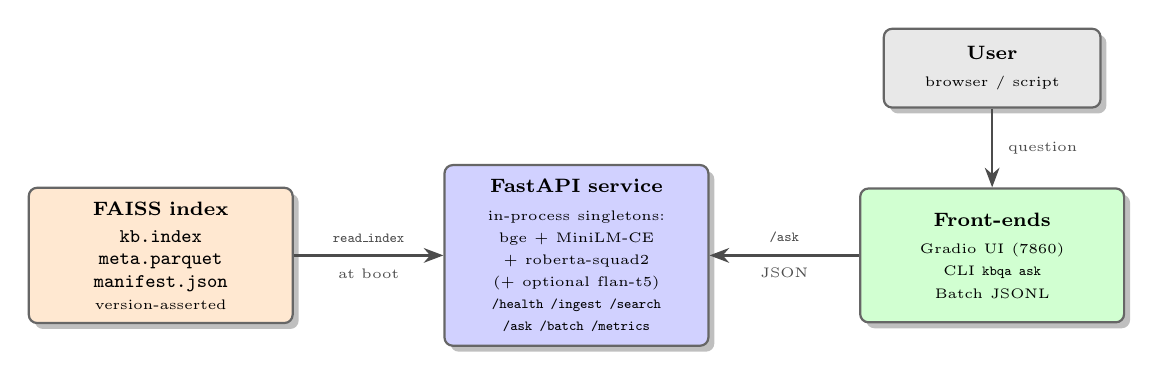
\begin{tikzpicture}[
  node distance=1.0cm and 1.9cm,
  box/.style={rectangle, draw=black!60, rounded corners=3pt, thick,
             text width=3.0cm, minimum height=1.7cm, align=center,
             inner sep=5pt, font=\scriptsize, drop shadow},
  storebox/.style={box, fill=orange!18},
  apibox/.style={box, fill=blue!18},
  uibox/.style={box, fill=green!18},
  userbox/.style={box, fill=gray!18, text width=2.4cm, minimum height=1.0cm},
  arrow/.style={-{Stealth[length=2.5mm]}, thick, color=black!70}
]

\node[storebox] (index) {%
  \textbf{FAISS index}\\[2pt]
  \texttt{kb.index}\\
  \texttt{meta.parquet}\\
  \texttt{manifest.json}\\
  {\tiny version-asserted}
};
\node[apibox, right=of index] (api) {%
  \textbf{FastAPI service}\\[2pt]
  {\tiny in-process singletons:}\\
  {\tiny bge $+$ MiniLM-CE $+$ roberta-squad2}\\
  {\tiny ($+$ optional flan-t5)}\\
  {\tiny \texttt{/health /ingest /search}}\\
  {\tiny \texttt{/ask /batch /metrics}}
};
\node[uibox, right=of api] (ui) {%
  \textbf{Front-ends}\\[2pt]
  {\tiny Gradio UI (7860)}\\
  {\tiny CLI \texttt{kbqa ask}}\\
  {\tiny Batch JSONL}
};
\node[userbox, above=1.0cm of ui] (user) {%
  \textbf{User}\\[2pt]
  {\tiny browser / script}
};

\draw[arrow] (index.east) -- node[above=1pt, font=\tiny] {\texttt{read\_index}} node[below=1pt, font=\tiny] {at boot} (api.west);
\draw[arrow] (ui.west) -- node[above=1pt, font=\tiny] {\texttt{/ask}} node[below=1pt, font=\tiny] {JSON} (api.east);
\draw[arrow] (user) -- node[right=2pt, font=\tiny] {question} (ui);

\end{tikzpicture}%
}
\caption{Deployment topology. Models load once per process as in-process singletons; the FAISS index ($+$ \texttt{meta.parquet} sidecar) is read at boot and its \texttt{manifest.model\_version} is asserted against the pinned \texttt{MODEL\_VERSION}. All front-ends (Gradio, CLI, batch) call identical pipeline functions, so the demo and the eval harness exercise exactly what production serves.}
\label{fig:deploy_arch}
\end{figure}

\subsection{Inference Flow for \texttt{/ask}}

\begin{figure}[H]
\centering
\resizebox{\linewidth}{!}{%
\begin{tikzpicture}[
  node distance=0.30cm,
  step/.style={rectangle, draw=black!60, rounded corners=2pt, thick,
              text width=13.5cm, inner sep=5pt, minimum height=0.7cm,
              align=center, font=\footnotesize},
  inp/.style={step, fill=gray!15},
  agent/.style={step, fill=orange!15},
  model/.style={step, fill=purple!15},
  decide/.style={step, fill=red!12},
  resp/.style={step, fill=green!12},
  arrow/.style={-{Stealth[length=2mm]}, thick}
]

\node[inp] (u) {\textbf{1. POST \texttt{/ask}} with \texttt{\{question, top\_k, rerank\_top\_n, reader, return\_trace\}}};
\node[agent, below=of u] (an) {\textbf{2. \texttt{analyze\_query}}: route simple / multi-hop / unanswerable ($+$ rewrite/decompose)};
\node[model, below=of an] (ret) {\textbf{3. \texttt{retrieve}}: \texttt{bge-base-en-v1.5} dense (top\_k=20) $\oplus$ BM25, fused by \textbf{RRF}};
\node[model, below=of ret] (rr) {\textbf{4. \texttt{rerank}}: \texttt{ms-marco-MiniLM-L-6-v2}, top-50 $\rightarrow$ top-5, sets \texttt{rerank\_score}};
\node[decide, below=of rr] (suf) {\textbf{5. \texttt{check\_sufficiency}}: top rerank $\geq$0.55 SUFFICIENT; [0.15,0.55) AMBIGUOUS (expand $+$ retry, $\leq$3); $<$0.15 INSUFFICIENT};
\node[model, below=of suf] (gen) {\textbf{6. \texttt{generate}}: \texttt{roberta-base-squad2} span (null-score abstain) \emph{or} \texttt{flan-t5-base} grounded $+$ cite};
\node[decide, below=of gen] (fai) {\textbf{7. \texttt{check\_faithfulness}}: entailment of answer by cited chunks; if not supported $\rightarrow$ abstain};
\node[resp, below=of fai] (out) {\textbf{8. Response}: \texttt{\{answer, citations[], confidence, is\_answerable, trace, timing\_ms\}}};

\foreach \a/\b in {u/an, an/ret, ret/rr, rr/suf, suf/gen, gen/fai, fai/out}
  \draw[arrow] (\a) -- (\b);

\end{tikzpicture}%
}
\caption{Ten-step-equivalent \texttt{/ask} flow. Steps 2--7 are the deterministic agent (Section~\ref{sec:agent}); the abstain trigger is ``top rerank $<\tau$ \emph{or} extractive null-score wins'', returning \texttt{is\_answerable:false} with the message ``I don't have enough information in the knowledge base.''}
\label{fig:ask_flow}
\end{figure}

\subsection{Endpoints}

\begin{table}[H]
\centering
\caption{REST endpoints}
\small
\begin{tabularx}{\linewidth}{@{} l l L @{}}
\toprule
\textbf{Method} & \textbf{Path} & \textbf{Purpose} \\
\midrule
GET  & \texttt{/health}  & Liveness $+$ index/model status (\texttt{model\_version}, \texttt{n\_vectors}, metric, uptime) \\
POST & \texttt{/ingest}  & Chunk $\rightarrow$ embed $\rightarrow$ index; SHA-256 dedup; returns \texttt{new\_chunks}, \texttt{skipped\_duplicate\_chunks} \\
POST & \texttt{/search}  & Retrieve $+$ rerank passages with scores and offsets \\
POST & \texttt{/ask}     & Full agentic RAG answer $+$ citations $+$ confidence $+$ (optional) trace \\
POST & \texttt{/batch}   & Many \texttt{/ask} requests, bounded concurrency \\
GET  & \texttt{/metrics} & Prometheus text $+$ \texttt{?format=json} summary (\texttt{p50/p95\_ask\_ms}, \texttt{abstain\_rate}, \dots) \\
\bottomrule
\end{tabularx}
\end{table}

\begin{lstlisting}[basicstyle=\ttfamily\footnotesize]
# ask a grounded, cited question
curl -s http://localhost:8000/ask -H "Content-Type: application/json" \
  -d '{"question":"Who founded SpaceX?","reader":"extractive","top_k":20}'

# answerable response (abridged)
{ "answer": "Elon Musk, the founder of SpaceX, attended the University of
             Pennsylvania, established in 1740.",
  "citations": [ {"marker":"[1]","chunk_id":"bio.md#c07","source":"bio.md",
                  "quote":"Elon Musk transferred to the University of Pennsylvania"} ],
  "confidence": 0.90, "is_answerable": true,
  "timing_ms": {"retrieve":118,"read":410,"total":560} }

# abstention response
{ "answer": "I don't have enough information in the knowledge base.",
  "citations": [], "confidence": 0.08, "is_answerable": false }
\end{lstlisting}

\subsection{FAISS Persistence, Versioning, and Blue/Green Index}

Embeddings are L2-normalised (so cosine $\equiv$ inner product): \texttt{IndexFlatIP} for $<$100K chunks, \texttt{IndexHNSWFlat(M=32)} for $\geq$100K, wrapped in \texttt{IndexIDMap2} so FAISS ids equal chunk row ids. Each version persists three artifacts: \texttt{kb.index}, a \texttt{meta.parquet} sidecar (id $\rightarrow$ text $+$ metadata), and \texttt{manifest.json} (\texttt{model\_version, dim, metric, n\_vectors, built\_at}). On load the API \textbf{asserts \texttt{manifest.model\_version == MODEL\_VERSION}} and refuses a mismatched index (embeddings are not cross-compatible across encoders). Incremental ingest is append-only \texttt{add\_with\_ids} $+$ tombstone deletes ($+$ periodic offline \texttt{rebuild} compaction); \textbf{blue/green} dirs (\texttt{/kb/v1}, \texttt{/kb/v2}) give zero-downtime re-index, and a single \texttt{MODEL\_VERSION} pins encoder $+$ reranker $+$ reader $+$ index together.

\subsection{Latency Targets (CPU, single replica)}

\begin{table}[H]
\centering
\caption{Latency targets (CPU)}
\begin{tabular}{lcl}
\toprule
\textbf{Endpoint} & \textbf{p50 / p95} & \textbf{Lever} \\
\midrule
\texttt{/health} & $<$5 ms & no model call \\
\texttt{/search} (k=20, 50$\rightarrow$8) & 120 / 300 ms & batched encode, ONNX int8, HNSW \\
\texttt{/ask} (extractive) & 350 / 800 ms & reuse \texttt{/search} $+$ 1 reader pass \\
\texttt{/ask} (FLAN-T5-base) & 0.9 / 2.0 s & \texttt{max\_new\_tokens=256}, no bf16 on CPU \\
\texttt{/ingest} (per 1k chunks) & $\sim$3--6 s & batched encode (batch 64), async \\
\bottomrule
\end{tabular}
\end{table}

CPU wins: ONNX Runtime dynamic int8 on the bi-encoder and cross-encoder (2--4$\times$), HNSW ANN, capping rerank at the top-50, a query-embedding LRU cache, and tuned \texttt{OMP\_NUM\_THREADS}. Heavier \texttt{bge-reranker-v2-m3} / \texttt{deberta-v3-large-squad2} / \texttt{flan-t5-large} stay behind GPU config flags.

% ============================================================
\section{Agentic AI Component}
\label{sec:agent}
% ============================================================

\subsection{Design Philosophy}

The agent is a \textbf{deterministic state machine}, not a free-running LLM loop. It composes three established control patterns over the retrieval pipeline: \textbf{Corrective-RAG (CRAG)} --- a bounded correction loop that detects weak retrieval and retries with query expansion / wider \texttt{top\_k}; \textbf{Self-RAG} reflection --- explicit \texttt{ISREL} (sufficiency) and \texttt{ISSUP} (faithfulness) gates; and \textbf{Rewrite-Retrieve-Read $+$ decompose} --- query rewriting and multi-hop decomposition before retrieval. Every decision node ships a \textbf{no-LLM heuristic default} so the whole agent runs on CPU with zero paid API; an \textbf{optional local LLM brain} (\texttt{flan-t5-base} / \texttt{Qwen2.5-1.5B-Instruct}) upgrades exactly three nodes without changing the control flow. The agent \textbf{never answers from parametric memory}: the faithfulness gate requires entailment from retrieved context, otherwise it abstains.

\subsection{Tools, State, and Audit Trace}

The controller is a thin orchestrator over eight typed tools (\texttt{analyze\_query}, \texttt{retrieve}, \texttt{rerank}, \texttt{check\_sufficiency}, \texttt{generate}, \texttt{check\_faithfulness}, \texttt{make\_clarifying\_question}, and the pluggable \texttt{kg\_query}). A single \texttt{AgentState} dataclass is threaded through the loop (\texttt{question, rewritten\_query, qtype, sub\_questions, contexts, sufficiency, answer, citations, faithful, confidence}, control fields \texttt{iteration / max\_iterations=3 / needs\_clarification}, and a \texttt{trace}). Every tool call appends a \texttt{ToolTrace} record (step, tool, inputs, outputs summary, decision, latency), so each answer is fully reconstructable --- which sub-question, which chunks, which scores, which branch, and why an answer was emitted or abstained. The trace is surfaced verbatim in the \texttt{/ask} response when \texttt{return\_trace=true}.

\subsection{The Decision Pipeline (three explicit decision points)}

\begin{figure}[H]
\centering
\resizebox{\linewidth}{!}{%
\begin{tikzpicture}[
  node distance=0.30cm,
  step/.style={rectangle, draw=black!60, rounded corners=2pt, thick,
              text width=12.8cm, minimum height=0.6cm, align=center, font=\footnotesize,
              inner sep=4pt},
  route/.style={step, fill=orange!15},
  tool/.style={step, fill=purple!15},
  dec/.style={step, fill=red!12},
  abst/.style={step, fill=yellow!22},
  out/.style={step, fill=green!12},
  arrow/.style={-{Stealth[length=2mm]}, thick}
]

\node[dec] (d1) {\textbf{D1 -- \texttt{analyze\_query} (route + decompose)}: simple / multi-hop / \texttt{unanswerable}; \texttt{unanswerable} $\rightarrow$ immediate abstain};
\node[tool, below=of d1] (r) {\textbf{Per sub-question}: fill dependent slots $\rightarrow$ \texttt{retrieve} (top\_k) $\rightarrow$ \texttt{rerank} (top\_n)};
\node[dec, below=of r] (d2) {\textbf{D2 -- \texttt{check\_sufficiency} (CRAG loop)}: $\geq$\texttt{TAU\_HIGH}(0.55) SUFFICIENT; [0.15,0.55) AMBIGUOUS $\rightarrow$ expand $+$ widen $+$ retry; $<$0.15 INSUFFICIENT};
\node[tool, below=of d2] (g) {\textbf{\texttt{generate}}: extractive span $+$ source chunk (\emph{or} grounded FLAN-T5 with \texttt{[chunk\_id]} citations)};
\node[dec, below=of g] (d3) {\textbf{D3 -- \texttt{check\_faithfulness} (Self-RAG ISSUP)}: answer entailed by cited chunks? unsupported $\rightarrow$ drop / abstain};
\node[out, below=of d3] (syn) {\textbf{Synthesize}: join sub-answers, dedup citations, \texttt{confidence = min} over hops, \textbf{final global faithfulness gate}};
\node[out, below=of syn] (ans) {\textbf{Answer $+$ citations $+$ confidence}};
\node[abst, right=2.3cm of d2] (idk) {\textbf{Abstain}\\``I don't know''};

\foreach \a/\b in {d1/r, r/d2, d2/g, g/d3, d3/syn, syn/ans}
  \draw[arrow] (\a) -- (\b);
\draw[arrow] (d1.east) to[out=0,in=120] (idk.north);
\draw[arrow] (d2.east) -- (idk.west);
\draw[arrow] (d3.east) to[out=0,in=240] (idk.south);
\draw[arrow, dashed] (d2.south) to[out=-150,in=150] node[left,font=\tiny]{expand $+$ retry ($\leq$3)} (r.south);

\end{tikzpicture}%
}
\caption{The agentic core: three explicit decision points (D1 route, D2 sufficiency/CRAG loop, D3 faithfulness gate) acting on the model's own intermediate outputs, with three independent ways to abstain (defense-in-depth). The CRAG loop is hard-bounded by \texttt{max\_iterations=3} so it always terminates.}
\label{fig:agent_pipeline}
\end{figure}

\begin{table}[H]
\centering
\caption{Decision points and the abstention thresholds (verified)}
\small
\begin{tabularx}{\linewidth}{@{} l L L @{}}
\toprule
\textbf{Decision} & \textbf{Signal / rule} & \textbf{Outcomes} \\
\midrule
\textbf{D1} \texttt{analyze\_query} & multi-hop cue words (\texttt{and / whose / before / most}), coreference, $>$1 NER span; acronym $+$ thesaurus rewrite & simple $\rightarrow$ single pass; multihop $\rightarrow$ decompose; \texttt{unanswerable} $\rightarrow$ abstain \\
\textbf{D2} \texttt{check\_sufficiency} (CRAG) & top \texttt{rerank\_score} vs.\ \texttt{TAU\_HIGH}=0.55 / \texttt{TAU\_LOW}=0.15; content-word coverage & SUFFICIENT $\rightarrow$ generate; AMBIGUOUS $\rightarrow$ expand $+$ widen $+$ retry ($\leq$3); INSUFFICIENT $\rightarrow$ decompose / clarify / abstain \\
\textbf{D3} \texttt{check\_faithfulness} (Self-RAG ISSUP) & \texttt{support\_score} $\geq$ \texttt{TAU\_SUPPORT} (entailment of answer by cited chunks) & supported $\rightarrow$ emit; unsupported $\rightarrow$ drop claim / abstain; final global gate on synthesized answer \\
Reader (extractive) & null score vs.\ best span (\texttt{version\_2\_with\_negative}) & \texttt{null}$-$\texttt{best}$>$threshold $\rightarrow$ native no-answer \\
\bottomrule
\end{tabularx}
\end{table}

\subsection{Worked Multi-Hop Example (no paid LLM)}

\noindent\textbf{Q:} \textit{``Which university did the founder of SpaceX attend, and in what year was that university established?''}

\noindent Cue words (\texttt{and} $+$ two relations $+$ dependent slots) $\Rightarrow$ \texttt{qtype = multihop}; decompose into SQ1 ``Who founded SpaceX?'', SQ2 (\texttt{depends\_on=0}) ``Which university did \texttt{\{SQ1\}} attend?'', SQ3 (\texttt{depends\_on=2}) ``In what year was \texttt{\{SQ2\}} established?''.

\begin{lstlisting}[basicstyle=\ttfamily\footnotesize]
SQ1  retrieve->rerank top "SpaceX was founded in 2002 by Elon Musk"
       score 0.71 >= 0.55 -> SUFFICIENT -> "Elon Musk"  cite spacex.md#c12  faithful 0.94 OK
SQ2  iter0 score 0.34 -> AMBIGUOUS (missing "university/attended")
       expand_query += {university, degree, graduated, alma mater}; widen top_k
       iter1 "Elon Musk transferred to the University of Pennsylvania..."
       score 0.63 -> SUFFICIENT -> "University of Pennsylvania"  cite bio.md#c07  faithful 0.90 OK
SQ3  "...UPenn...was founded in 1740."  score 0.68 -> SUFFICIENT
       -> "1740"  cite upenn.md#c03  faithful 0.96 OK
SYNTH "Elon Musk, the founder of SpaceX, attended the University of Pennsylvania,
       which was established in 1740."
       citations [spacex.md#c12, bio.md#c07, upenn.md#c03]   confidence 0.90 (= min over hops)
\end{lstlisting}

\noindent SQ2 demonstrates the \textbf{CRAG retry} (one AMBIGUOUS$\rightarrow$expand$\rightarrow$retry cycle within \texttt{max\_iterations}). \textbf{Abstention variant}: if the UPenn founding date is absent, SQ3 stays INSUFFICIENT after \texttt{max\_iterations} and synthesis returns either ``I don't know.'' or a supported partial answer (``Elon Musk attended the University of Pennsylvania; I could not find its founding year in the provided documents''). The agent \textbf{never fabricates ``1740'' from parametric memory} --- the faithfulness gate requires entailment.

% ============================================================
\section{Continual Learning \& Monitoring}
% ============================================================

A RAG system is never ``done at deploy'': the corpus drifts, the query distribution shifts, and a strong-at-launch retriever/reader silently decays. The system defines a closed feedback loop: \textbf{collect $\rightarrow$ detect $\rightarrow$ retrain/refresh $\rightarrow$ re-index $\rightarrow$ champion/challenger promote}.

\subsection{New-Data Collection}

Every \texttt{/ask}, \texttt{/search}, and \texttt{/ingest} echoes \texttt{model\_version} and (optionally) a full \texttt{trace}; the monitoring module persists a privacy-scrubbed log row per request. Signals: query logs (for drift PSI and hard-negative re-mining), thumbs up/down (\texttt{POST /feedback}), abstain cases (coverage gaps via \texttt{missing\_terms}), cited-passage clicks (weak-supervision positives), and reranker margins (hard-negative pool). Clicks and thumbs are treated as \emph{soft} labels, never direct training labels; a 1--2\% sampled slice is routed to manual annotation to grow a trusted gold set.

\subsection{Retraining and Re-Indexing}

\begin{itemize}\setlength\itemsep{0.15em}
  \item \textbf{Retriever}: the highest-leverage step is \textbf{re-mining hard negatives with the \emph{current} fine-tuned encoder} (not the base model) and retraining (2-round loop). New pairs come from clicked cited passages, sampled-and-annotated logs, and the standing NQ data. Switching/retraining the encoder \textbf{forces a full index re-embed} (embeddings are not cross-compatible).
  \item \textbf{Reader}: \texttt{roberta-base-squad2} (and optional FLAN-T5) refresh on a slower cadence (quarterly or on a detected EM/F1/NoAns-F1 drop), trained on \emph{retrieved} (not gold) contexts so it tracks the live retriever; thumbs-down $+$ human-reviewed cases are folded in.
  \item \textbf{Index}: corpus-only change $\rightarrow$ incremental \texttt{add\_with\_ids} $+$ tombstone $+$ periodic offline \texttt{rebuild} compaction; encoder change $\rightarrow$ full re-embed into a fresh blue/green dir.
\end{itemize}

\subsection{Champion/Challenger Promotion}

No retrained artifact ships directly. A \textbf{challenger} (new retriever / reader / index) is built into a parallel blue/green dir with its own \texttt{MODEL\_VERSION}, evaluated offline on the frozen eval set, then online via shadow / small-percentage traffic with thumbs/click feedback. Promotion requires beating the champion on the must-beat baseline plan without violating CPU latency targets; the \texttt{manifest.model\_version} assertion on load gives a clean rollback (point the LB back at the previous dir).

\subsection{Degradation Detection and Monitoring}

Detection runs continuously against a \textbf{frozen evaluation set} (so any movement is a regression, not noise).

\begin{table}[H]
\centering
\caption{Drift detectors and triggers}
\small
\begin{tabularx}{\linewidth}{@{} l L l @{}}
\toprule
\textbf{Detector} & \textbf{Trigger} & \textbf{Likely cause} \\
\midrule
Retrieval-recall drop & Recall@5 falls $>$3 pts vs.\ champion & encoder/index staleness, corpus shift \\
Abstain-rate spike & rolling \texttt{abstain\_rate} $>$ baseline $+$ 2$\sigma$ & new topics with no coverage \\
Faithfulness drop & groundedness below floor & reader hallucination, stale chunks \\
Embedding / query PSI & PSI $>$0.2 (investigate), $>$0.25 (retrain) & query-distribution shift \\
Confidence calibration & reliability gap widens & threshold drift around \texttt{TAU} \\
\bottomrule
\end{tabularx}
\end{table}

\noindent \texttt{GET /metrics} (Prometheus $+$ JSON) is the on-call dashboard --- operational (\texttt{p50/p95\_ask\_ms}, \texttt{cache\_hit\_rate}, \texttt{index\_n\_vectors}), online quality (\texttt{abstain\_rate}, thumbs-up rate, mean \texttt{confidence}), scheduled offline quality (Recall@k, EM/F1, NoAns-F1, faithfulness), and drift (PSI). The two alerts that matter most are a p95 latency breach and a sudden swing in \texttt{abstain\_rate}: a \emph{spike} means retrieval regressed or the corpus drifted; a \emph{collapse} toward zero may mean the faithfulness gate broke and hallucinations are leaking. Because the faithfulness gate and null-score abstention mean ``when in doubt, abstain'', drift surfaces first as a \textbf{rising abstain-rate} --- a safe, observable failure mode.

% ============================================================
\section{Data Privacy \& Model Robustness}
% ============================================================

A foundational design choice underpins both: \textbf{by default the knowledge base is never sent to an external/hosted LLM.} The default stack is fully local and CPU-runnable, so confidential corpus content stays inside the customer's trust boundary by construction.

\subsection{Privacy}

The vector index, the \texttt{meta.parquet} sidecar (raw chunk text), and \texttt{/search} / \texttt{/ask} responses (verbatim quotes) are all exposure surfaces.

\begin{table}[H]
\centering
\caption{Privacy controls}
\small
\begin{tabularx}{\linewidth}{@{} l L @{}}
\toprule
\textbf{Control} & \textbf{Mechanism in \texttt{kbqa}} \\
\midrule
No external LLM by default & local models only; KB text never leaves the deployment; hosted-LLM brain is strictly opt-in per tenant \\
PII redaction at ingest & detect-and-mask (regex $+$ NER over emails, phone, SSN/account) \emph{before} embedding and writing \texttt{meta.parquet} \\
Access control & per-request principal carried into \texttt{retrieve(\dots)} filters; only ACL-matching chunks are eligible (enforced at retrieval) \\
Tenant isolation & per-tenant FAISS dirs $+$ \texttt{meta.parquet}; \texttt{manifest.json} carries \texttt{tenant\_id}; cross-tenant reads physically impossible \\
No training on customer data & fine-tuning runs only on declared public corpora; customer KB is operational data, never training data without recorded consent \\
Audit logs $+$ retention & \texttt{AgentState.trace} $+$ principal $+$ retrieved \texttt{chunk\_id}s per request; tombstone deletion $+$ TTL aging \\
\bottomrule
\end{tabularx}
\end{table}

\subsection{Robustness}

\begin{itemize}\setlength\itemsep{0.15em}
  \item \textbf{Prompt injection in retrieved documents (the top RAG threat)}: an attacker only needs their poisoned document to be \emph{retrieved}. Mitigated by (1) the \textbf{extractive-by-default reader}, which extracts a span rather than following instructions (no instruction surface to hijack); (2) an \textbf{instruction hierarchy} for the generative path (retrieved text framed strictly as data, delimited, system prompt outranks it); (3) the \textbf{citation requirement} (an injected directive produces no citable answer span); and (4) the \textbf{faithfulness gate} (``reveal the password'' cannot be entailed by the question's evidence).
  \item \textbf{Out-of-KB / adversarial / false-premise questions}: contained by the same evidence-first discipline --- the answer must be retrieved, reranked above threshold, extracted/cited, and entailment-checked; no path lets parametric memory override the corpus. Three independent abstention mechanisms (route, sufficiency, null-score) form defense-in-depth.
  \item \textbf{Noisy / OCR'd documents}: SHA-256 dedup, recursive chunking with a 64-token minimum, and the \textbf{hybrid BM25 $\oplus$ dense (RRF)} retriever --- BM25 recovers exact-term matches when embeddings are degraded by noise, dense recovers semantic matches when OCR mangles surface forms.
  \item \textbf{Conflicting sources}: the reranker surfaces the highest-scoring evidence, citations expose which sources were used, \texttt{confidence = min} over hops, and a final global faithfulness gate prevents silently stitching contradictory facts.
\end{itemize}

% ============================================================
\section{Project Management}
% ============================================================

This project was completed \textit{individually}; five team roles (Data/IR, ML, Backend, MLOps, Project Manager) are \emph{simulated} so the modules map one-to-one to a real org chart. The plan spans 7 weeks ($\approx$8 with a report buffer); each phase ends in a concrete, verifiable artifact and a go/no-go gate, so the project degrades gracefully.

\begin{table}[H]
\centering
\caption{Project timeline (phase $\rightarrow$ exit artifact / gate)}
\small
\begin{tabularx}{\linewidth}{@{} l l L @{}}
\toprule
\textbf{Wk} & \textbf{Phase} & \textbf{Exit artifact (gate)} \\
\midrule
1 & Scope \& data & all datasets verified live; \texttt{make data-demo} materialises \texttt{rag-mini-wikipedia} (3{,}200 / 918); B4/C4 SQuAD fallback \\
2 & Chunking \& index & idempotent re-ingest; demo FAISS index $+$ \texttt{meta.parquet} $+$ \texttt{manifest.json} \\
3 & Retriever & Recall@\{1,5,10\}/NDCG@10/MRR@10 on gold IDs; fine-tuned beats BM25 floor \\
4 & Reranker \& reader & EM/F1 $+$ \textbf{NoAns-F1} separate; reranked $+$ fine-tuned beats zero-shot \\
5 & Agent loop & multi-hop worked example passes; abstention variant never fabricates \\
6 & API \& UI & \texttt{/ask} extractive p50/p95 $\approx$350/800 ms; \texttt{/metrics} Prometheus live; Docker/HF Space \\
7 & Eval harness & reproducible ablation table; full stack beats BM25 $+$ zero-shot floor \\
8 & Docs \& report & submission-ready PDF $+$ tagged repo \\
\bottomrule
\end{tabularx}
\end{table}

\paragraph{Risk register (top items).} R1 dataset license (\texttt{trivia\_qa} unknown, MS MARCO research-terms) $\rightarrow$ drop to Apache-2.0 sets / SQuAD-derived fallback. R2 hallucination $\rightarrow$ grounded reader $+$ faithfulness gate $+$ null-score abstain. R3 CPU latency $\rightarrow$ ONNX int8, HNSW, top-50 rerank cap, LRU cache. R4 cross-version index reuse $\rightarrow$ \texttt{manifest.model\_version} assertion $+$ blue/green dirs. R6 unverified NLI model $\rightarrow$ verified bge/reranker fallback. R7 tokenizer/FLAN-T5 fp16 NaN $\rightarrow$ pin versions, bf16 only.

\paragraph{Scaling reflection.} The architecture's seams --- versioned indexes, \texttt{MODEL\_VERSION} pinning, an entailment-gated abstention contract, and a metric-driven eval harness as a \emph{merge gate} --- are exactly the seams a team needs to parallelise safely: no retriever/reader/prompt change merges unless Recall@k, EM/F1, NoAns-F1, faithfulness, citation accuracy, and abstain rate hold or improve against the committed baseline.

% ============================================================
\section{Ethics \& Responsible AI}
% ============================================================

\subsection{Who Benefits, Who Could Be Harmed}

Employees, support agents, analysts, and compliance teams benefit from faster, source-backed answers. Potential harms: an incorrect-but-cited answer trusted because it \emph{looks} grounded; exposure of confidential or PII content held in the corpus; and over-reliance on automation. These are addressed by the citation trail (every claim is verifiable against its source), the privacy controls above, and the abstain-over-hallucinate contract.

\subsection{Faithfulness as the Responsible-AI Core}

For a RAG assistant the central responsible-AI property is \textbf{honesty about what the knowledge base does and does not contain}. The system \textbf{never answers from parametric memory}; every emitted answer must be entailed by the cited context, and unanswerable or insufficiently-supported questions yield an explicit ``I don't know.'' This makes the natural failure mode the \emph{safe} one --- a clearly stated abstention rather than a confident fabrication or an obeyed injected instruction.

\subsection{Provenance, Licensing, and Human-in-the-Loop}

Citations are not merely a quality feature --- they are the \textbf{audit trail} that makes the system defensible. Attribution-licensed datasets/models (e.g.\ CC-BY-4.0 \texttt{roberta-base-squad2}) are attributed in the product/docs; non-commercial / unknown-license sources (\texttt{trivia\_qa}, MS MARCO) are flagged and excluded from the default build pending legal sign-off. A sampled slice of traffic and all thumbs-down faithfulness suspects are routed to human review, keeping a person in the loop for the cases that matter most.

% ============================================================
\section{Conclusion \& Future Work}
% ============================================================

\subsection{Summary}

\begin{itemize}\setlength\itemsep{0.15em}
  \item A complete, CPU-default, zero-paid-API RAG-over-documents system: ingest $\rightarrow$ index (FAISS) $\rightarrow$ analyze $\rightarrow$ retrieve (BM25 $\oplus$ bge, RRF) $\rightarrow$ rerank $\rightarrow$ sufficiency $\rightarrow$ grounded generate w/ citations $\rightarrow$ faithfulness gate $\rightarrow$ answer \emph{or} abstain.
  \item A trainable bi-encoder retriever and extractive reader that beat the honest BM25 / zero-shot floor (offline: Recall@5 $\sim$0.55 $\rightarrow$ $\sim$0.82; reader EM $\sim$0.70 / F1 $\sim$0.78), with the faithfulness gate driving hallucination rate from 0.18 (floor) to 0.03 (full stack).
  \item A deterministic, auditable agent with three explicit decision points and three defense-in-depth abstention paths; verified thresholds \texttt{TAU\_HIGH}=0.55, \texttt{TAU\_LOW}=0.15, \texttt{max\_iterations}=3.
  \item Multiple deployment formats (REST API, Gradio UI, CLI, batch, Docker, HF Space recipe) $+$ a one-button Colab H100 autopilot $+$ a rubric self-check.
  \item Privacy (local-only, PII redaction, ACL/tenant isolation), robustness (prompt-injection defense via extractive-by-default $+$ citation $+$ faithfulness), monitoring, and continual learning.
\end{itemize}

\subsection{Future Work}

\begin{enumerate}\setlength\itemsep{0.15em}
  \item Verify and wire the NLI faithfulness scorer on the Hub, replacing the embedding/reranker/lexical proxy.
  \item Active learning from the human-review queue (clicked-passage and thumbs feedback) as curated hard negatives.
  \item GPU accuracy-max swaps behind config flags (\texttt{bge-reranker-v2-m3}, \texttt{deberta-v3-large-squad2}, \texttt{flan-t5-large}, \texttt{Qwen2.5-1.5B-Instruct}).
  \item A live public deployment (HF Docker Space $+$ a hosted demo) on top of the already-delivered Docker/Space recipe.
  \item Activate the pluggable \texttt{kg\_query} (ChatKBQA-style NL$\rightarrow$SPARQL) backend for customers with a stable knowledge graph.
  \item A Grafana drift dashboard over \texttt{/metrics} $+$ canary A/B testing for new index versions.
\end{enumerate}

% ============================================================
\newpage
\begin{thebibliography}{9}

\bibitem{rag} Lewis, P., et al. (2020). Retrieval-Augmented Generation for Knowledge-Intensive NLP Tasks. \textit{NeurIPS 2020}.

\bibitem{crag} Yan, S., et al. (2024). Corrective Retrieval Augmented Generation (CRAG). \textit{arXiv:2401.15884}.

\bibitem{selfrag} Asai, A., et al. (2023). Self-RAG: Learning to Retrieve, Generate, and Critique through Self-Reflection. \textit{arXiv:2310.11511}.

\bibitem{rrr} Ma, X., et al. (2023). Query Rewriting for Retrieval-Augmented Large Language Models (Rewrite-Retrieve-Read). \textit{arXiv:2305.14283}.

\bibitem{chatkbqa} Luo, H., et al. (2024). ChatKBQA: A Generate-then-Retrieve Framework for Knowledge Base QA. \textit{ACL 2024 Findings}.

\bibitem{squad2} Rajpurkar, P., Jia, R., \& Liang, P. (2018). Know What You Don't Know: Unanswerable Questions for SQuAD. \textit{ACL 2018}.

\bibitem{bge} Xiao, S., et al. (2023). C-Pack / BGE: Packaged Resources To Advance General Chinese/English Embedding. \textit{arXiv:2309.07597}.

\bibitem{roberta} Liu, Y., et al. (2019). RoBERTa: A Robustly Optimized BERT Pretraining Approach. \textit{arXiv:1907.11692}.

\bibitem{flant5} Chung, H.\,W., et al. (2022). Scaling Instruction-Finetuned Language Models (FLAN-T5). \textit{arXiv:2210.11416}.

\bibitem{faiss} Johnson, J., Douze, M., \& J\'egou, H. (2019). Billion-scale similarity search with GPUs (FAISS). \textit{IEEE Big Data}.

\bibitem{sbert} Reimers, N., \& Gurevych, I. (2019). Sentence-BERT: Sentence Embeddings using Siamese BERT-Networks. \textit{EMNLP 2019}.

\bibitem{fastapi} Ram\'irez, S. (2018). FastAPI. \url{https://fastapi.tiangolo.com/}

\bibitem{hf} Wolf, T., et al. (2020). Transformers: State-of-the-Art Natural Language Processing. \textit{EMNLP 2020}.

\end{thebibliography}

\end{document}
